\section{Getting Started}
\label{sec:getting-started}

\subsection{Setup}
\label{sec:setup}

The Scenario Checker is installed into Rodin from the update site, \emph{Soton Plug-ins} in the normal way.
It is located under the category, \emph{Scenario Checker}.
The Scenario Checker depends on (and will install elements from)
\begin{itemize}
\item ProB - de.prob
\item ProB Support - ac.soton.eventb.probsupport
\item Event-B EMF framework - org.eventb.emf
\item Oracle - persistence for scenarios
\end{itemize}

\subsection{Perspective}
\label{sec:perspective}

The Scenario Checker defines a perspective (see Fig. \ref{fig:perspective}) which includes the Scenario Checker Control Panel view, the Scenario Checker State view and the Scenario Checker Console.
The upper editing panels can be used to show other state animation tools.
For example, in Fig. \ref{fig:perspective},  BMotionStudio and UML-B State-machine animations are shown.
The perspective also includes ProB views which are stacked behind the Scenario Checker views.
These can used to see the the state, enabled events and execution history in a more basic Event-B form if needed.

\begin{figure}[!htbp]
	\centering
	\ifplastex
	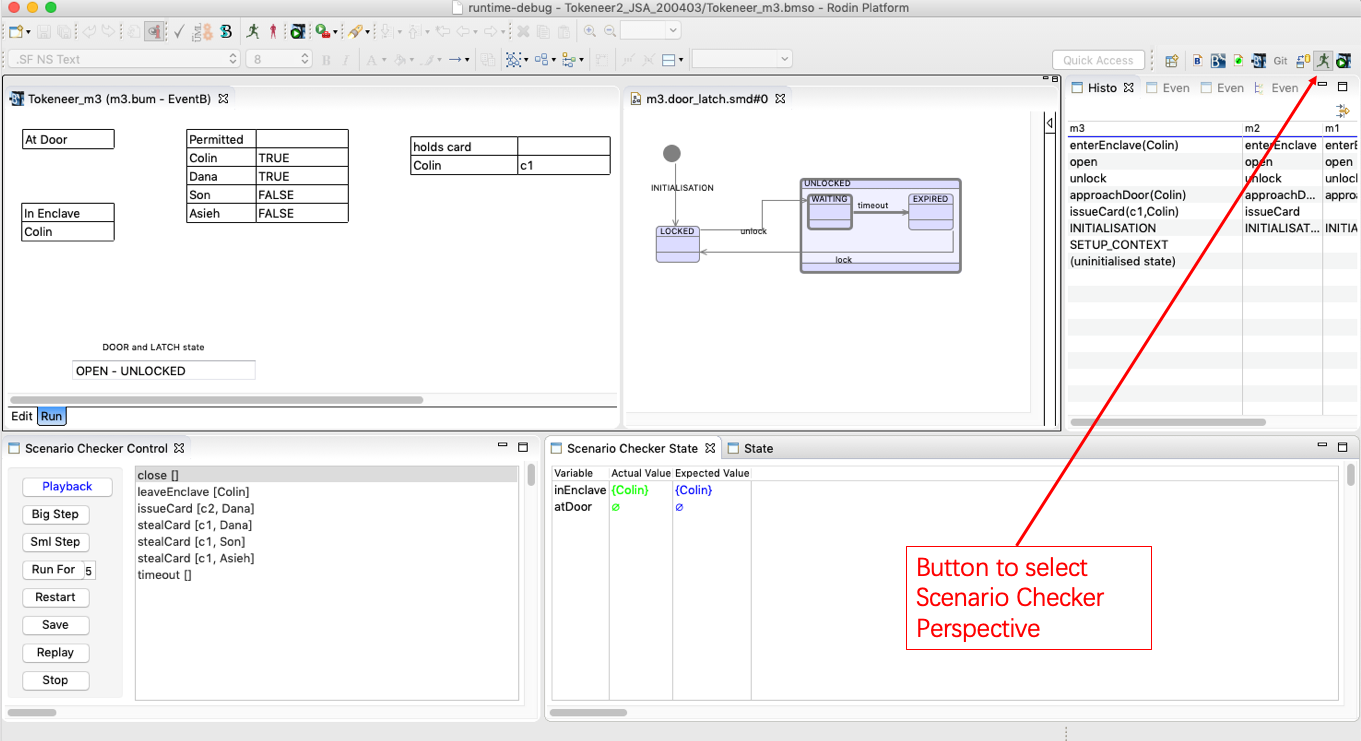
\includegraphics[width=900]{figures/perspective}
	\else
	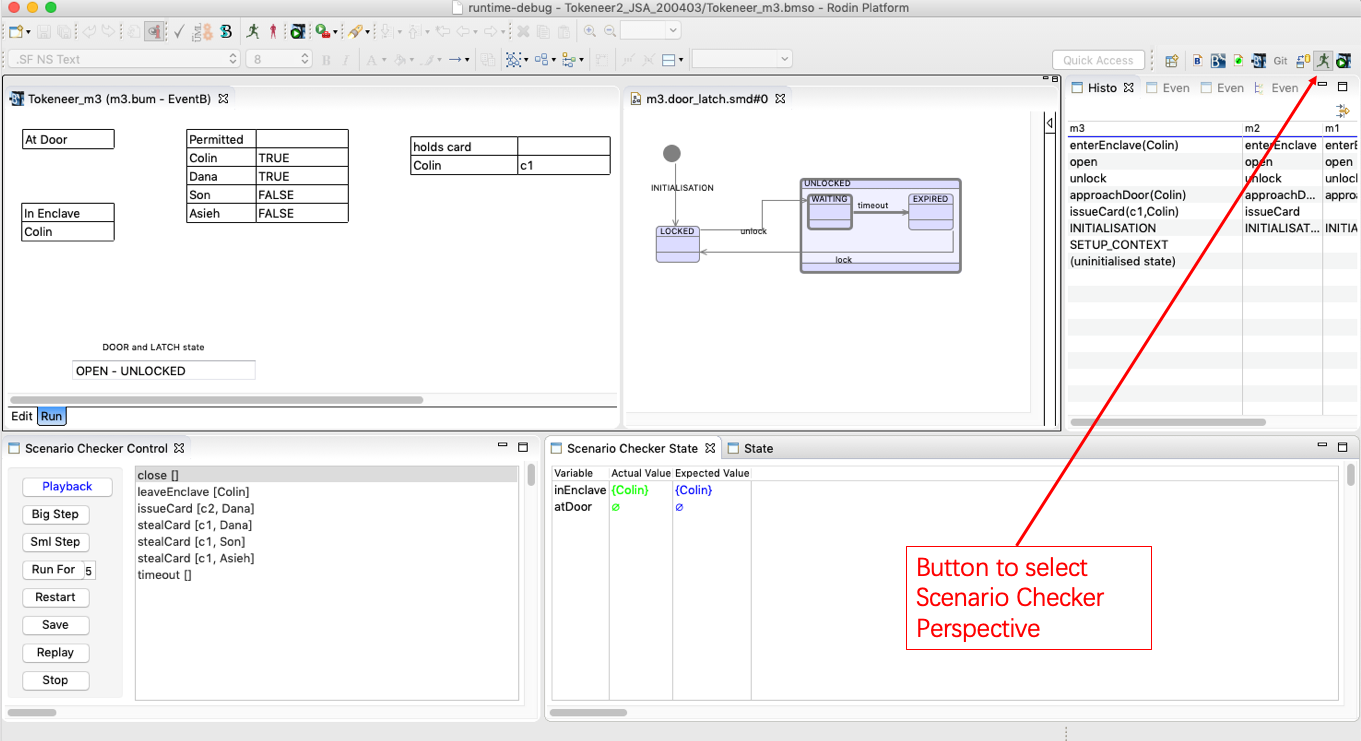
\includegraphics[width=0.9\textwidth]{figures/perspective}
	\fi
	\caption{Scenario Checker Perspective}
	\label{fig:perspective}
\end{figure}

The Scenario Checker views are also contributed to the BMotion Studio Run perspective and are available as short cuts on the Event-B perspective.

\subsection{Starting}
\label{sec:starting}

The Scenario Checker is started using the context menu of a machine as shown in Fig. \ref{fig:starting1}.
I.e. by right clicking on a machine in the Event-B navigator and selecting the \textbf{Scenario Checker} menu item.

\begin{figure}[!htbp]
	\centering
	\ifplastex
	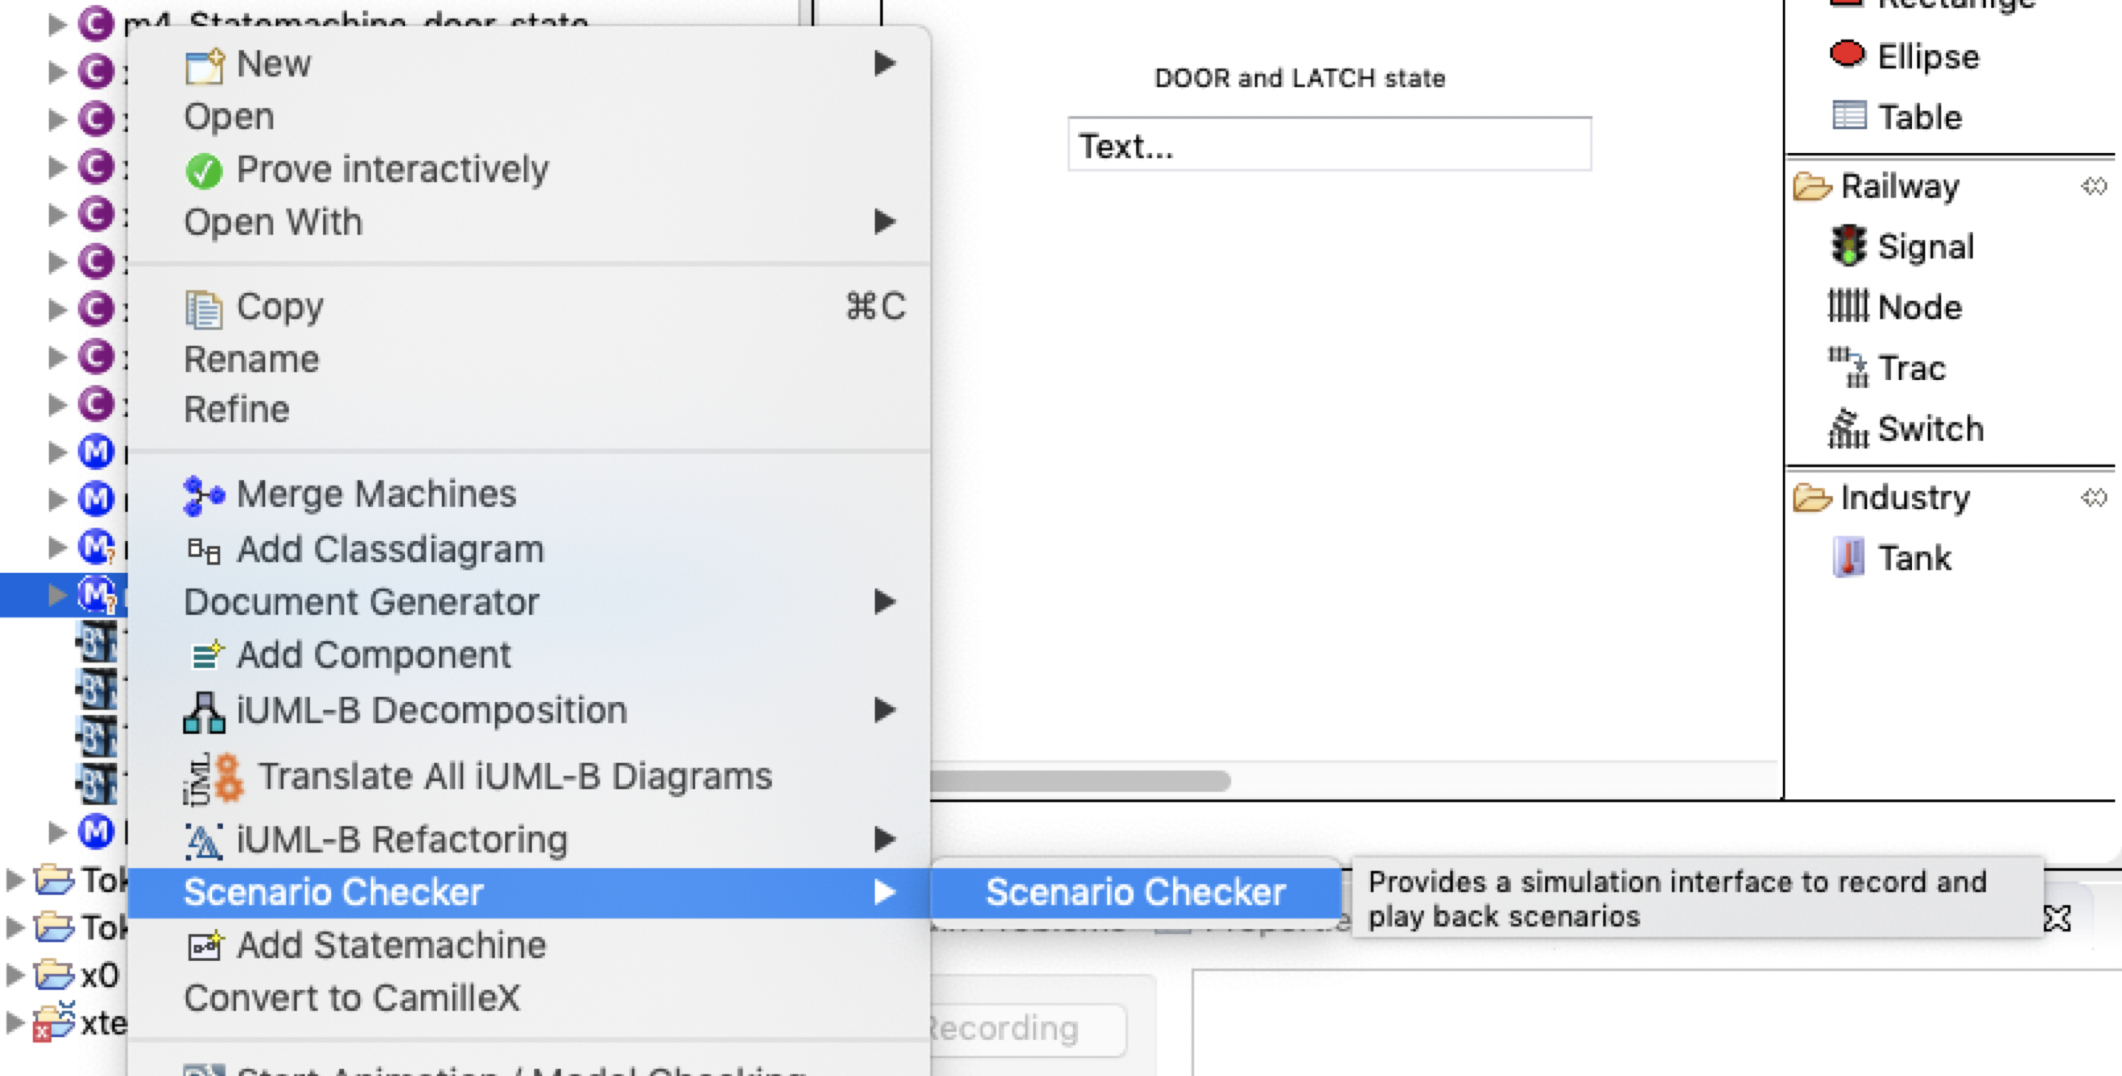
\includegraphics[width=700]{figures/starting1}
	\else
	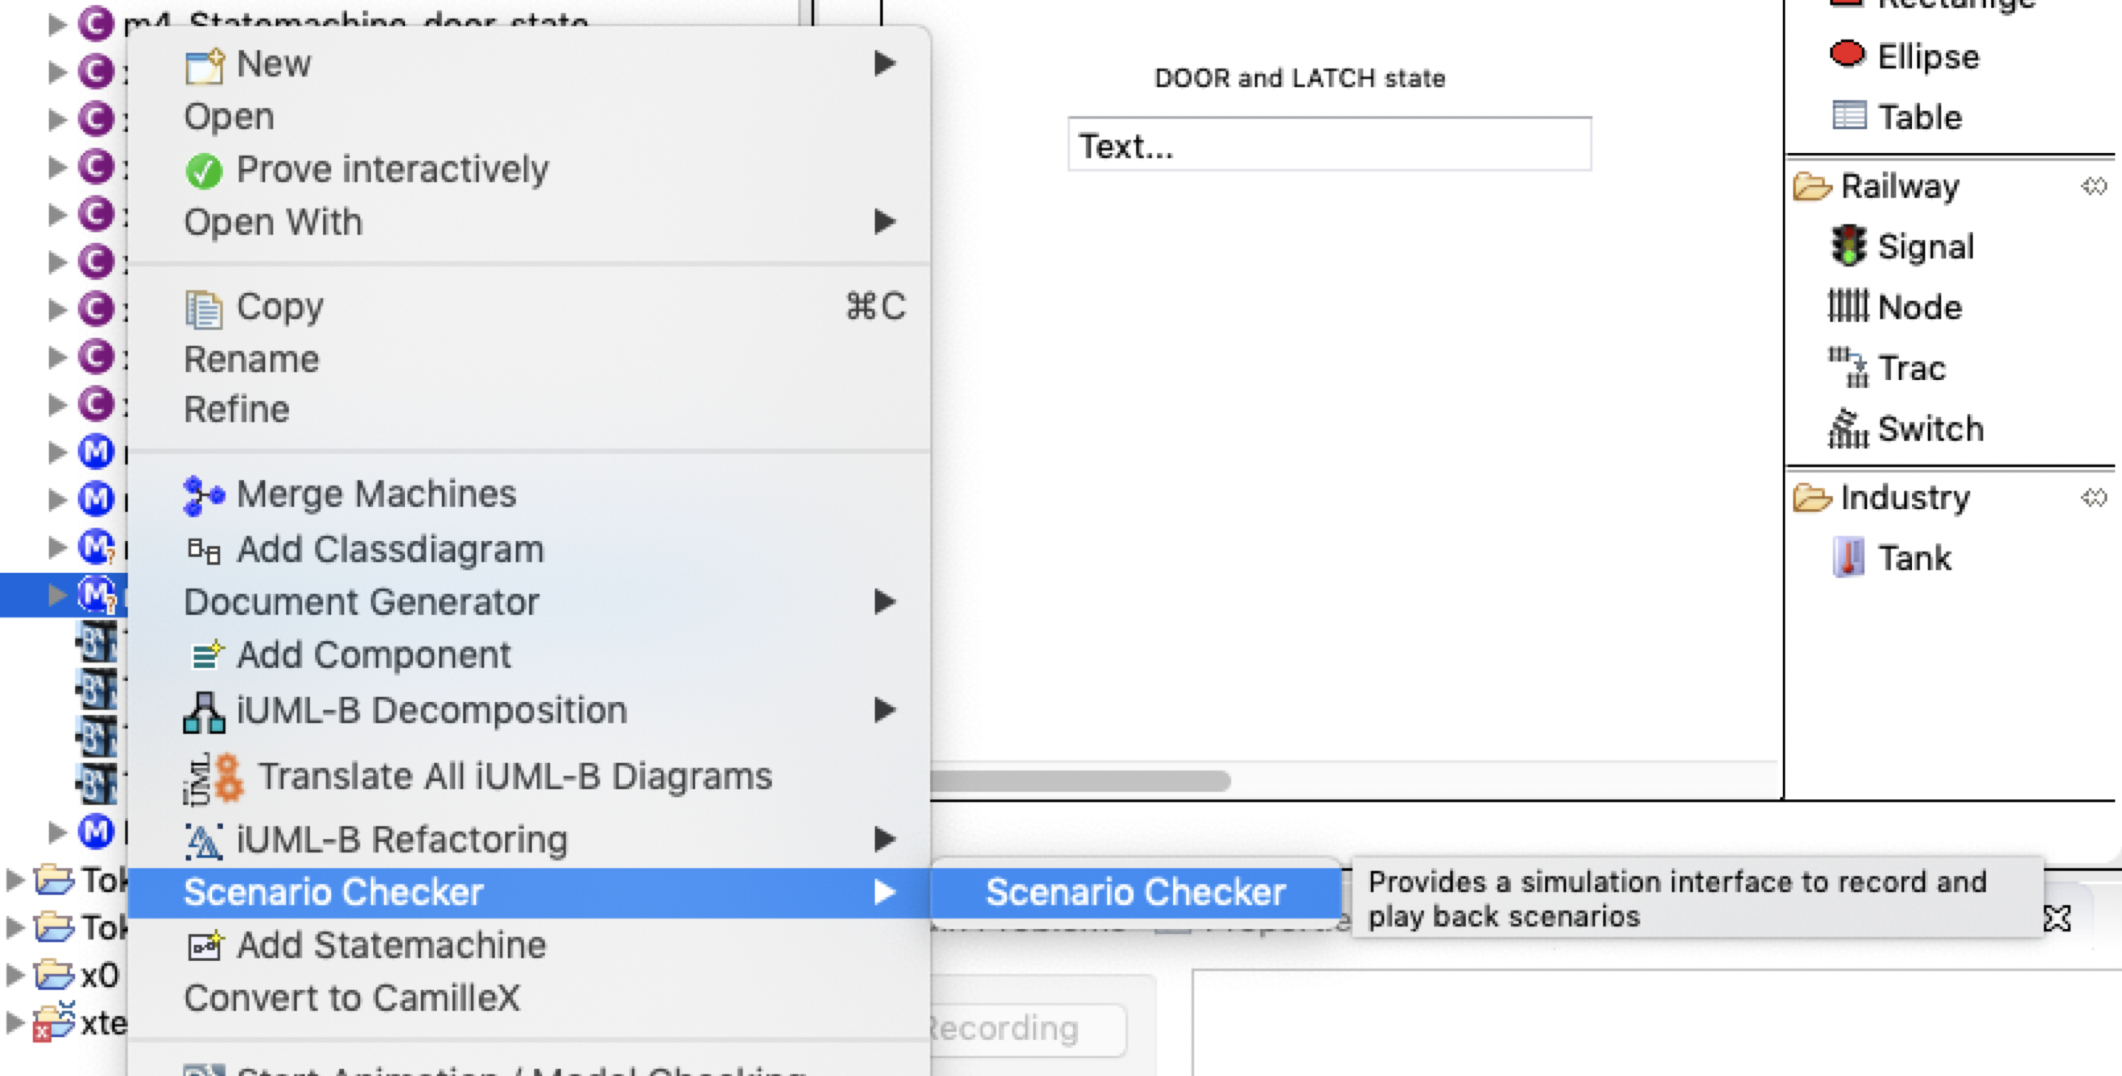
\includegraphics[width=0.75\textwidth]{figures/starting1}
	\fi
	\caption{Starting the Scenario Checker from the context menu}
	\label{fig:starting1}
\end{figure}

An alternative way to start the Scenario Checker is to ensure that at least one of the scenario views is opened (e.g. by selecting the Scenario Checker perspective) and then using the toolbar button of the ProB support plug-in (the green running man shown circled in red in \ref{fig:starting2}).

\begin{figure}[!htbp]
	\centering
	\ifplastex
	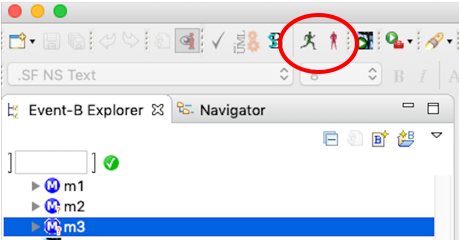
\includegraphics[width=400]{figures/starting2}
	\else
	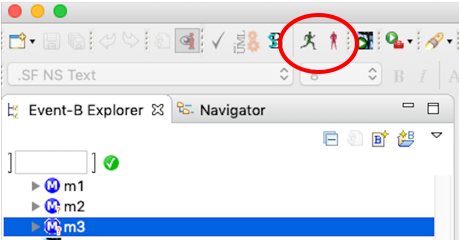
\includegraphics[width=0.4\textwidth]{figures/starting2}
	\fi
	\caption{Starting/Stopping the Scenario Checker using the toolbar icons}
	\label{fig:starting2}
\end{figure}

In either case, the ProB support plug-in will be used to simultaneously launch the scenario checker and any other participating animation plugins that are open for  the same machine.
For example, a BMotion Studio visualisation and/or a UML-B state-machine could be used to visualise the state of the model to assist validation.

The Scenario Checker is stopped by clicking the red standing man toolbar button. If another animation is started using the ProB support plugin, any current animation is aborted.

\subsection{Setup}
\label{sec:setup}

The Scenario Checker always fires the ProB setup operation whenever it can (i.e. when it is started or re-started or replayed).
It is important for the sets and constants in the model, to be instantiated with suitable values to record a desired scenario.
The same values must also be instantiated in order for previously recorded scenarios to be replayed.
This can be done by adding an animation context that is seen by the machine to be animated.

\subsection{Persistence}
\label{sec:persistence}

Scenarios are persisted in the Oracle format.
This is an XML based format consisting of two types of elements (Steps and Snapshots) which are expected to alternate.
A \textbf{Step} records the event signature that fired as part of the scenario.
A \textbf{Snapshot} records the state of any variables and constants that changed value as a result of the preceding step.
The first step is always the ProB \texttt{SETUP} operation and this is followed by the first snapshot giving the values of sets and constants.
The second step is the \texttt{INITIALISATION} followed by the snapshot giving the initial value of all variables.
After this the steps and snapshots depend on the scenario.
The oracle format is defined and generated from an EMF meta-model and hence is the default EMF XMI format for that meta-model.
Scenarios can be read and edited using an EMF editor such as Rose (available via the Soton Plug-ins update site).


%%% Local Variables:
%%% mode: latex
%%% TeX-master: "user_manual"
%%% End:
